\subsection{ResUNet}
The model is the following:
\begin{figure}[H]
    \centering
    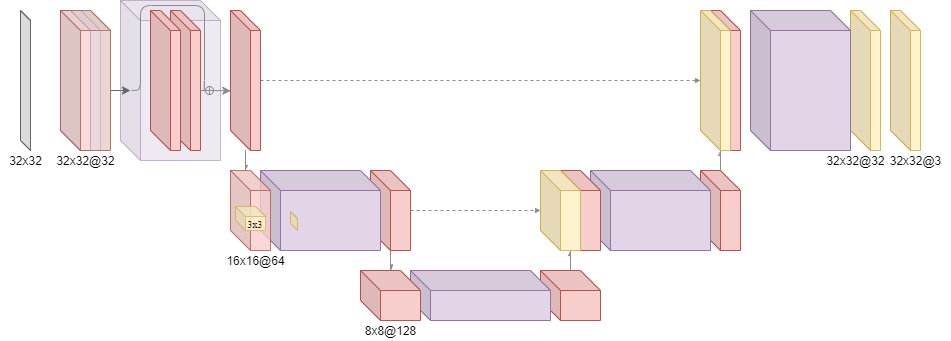
\includegraphics[scale=0.3]{subsections/resunet/resunet.png}
\end{figure}


The U-Net \cite{unet} architecture is largely used in image segmentation due to its structure: the descending path encodes the image information and the ascending path decode the information localized at particular position inside the ground truth image.

Descending and ascending paths are connected togheter at each level in order to share the information and achive a more precise classification: this is done \textit{concatenating} the features of each output in the descending path to the upsampled input of the ascending path.  

This pattern can be also used for image-to-image processing although some changes are necessary:
\begin{itemize}
    \item With respect to the original paper the downsampling and upsampling is done respectively using \textit{Conv2D}(red) and \textit{Conv2DTranspose}(yellow) in order to "learn" the transformation instead of using MaxPooling and UpSampling leading to a loss of information.
    \item Moreover the \textit{ResBlock} ( as defined in \cite{resnet} ) is used in order to increment the amount of information propagated at each level in both paths. \footnote{In the CAESSC network will be discussed the advantages of the residual connections}
\end{itemize}

Since this network was used with \textit{CIFAR10} only (allowing a large batch), the \textit{Conv2D} layer is composed by:
\begin{enumerate}
    \item Conv2D using a filter $(3,3)$
    \item BatchNormalization \cite{BN}. It's necessary since the batch size is huge thus it allow to maintain the distribution of the inputs on each layer for each batch the same, allowing a faster training using a higher learning rate and avoiding exploding/vanising gradients.
    \item Activation
\end{enumerate}

The \textit{ResBlock} is composed by two Conv2D layers and the output is the concatenation of the last output with the input.  

The networks implemented are: \textbf{ResUNet1} with 1 ResBlock and \textbf{ResUNet3} with 3 ResBlock.

\subsection{Training}
The network was trained with Adam\cite{adam} with default parameters using an early stopping equals to 7 for avoiding overfitting and MSE as loss function.
SRNDeblur1 and SRNDeblur3 converged, respectively, after 40 and 50 epochs.
\begin{figure}[H]
    \begin{subfigure}{\textwidth}
        \centering
        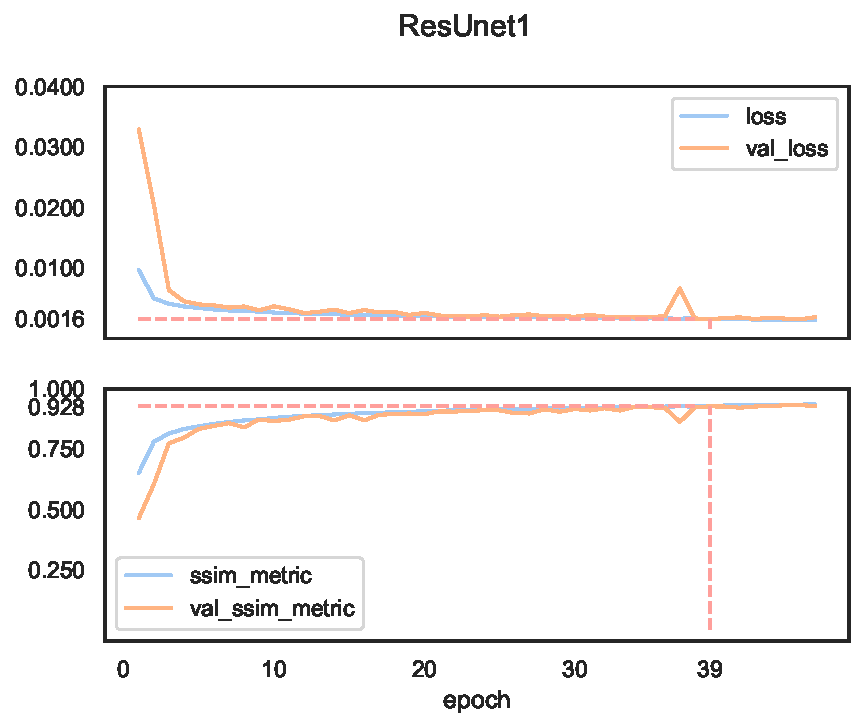
\includegraphics[height=0.4\textheight,keepaspectratio]{subsections/resunet/plot_history_ResUNet1.pdf}            
    \end{subfigure}
    \begin{subfigure}{\textwidth}
        \centering
        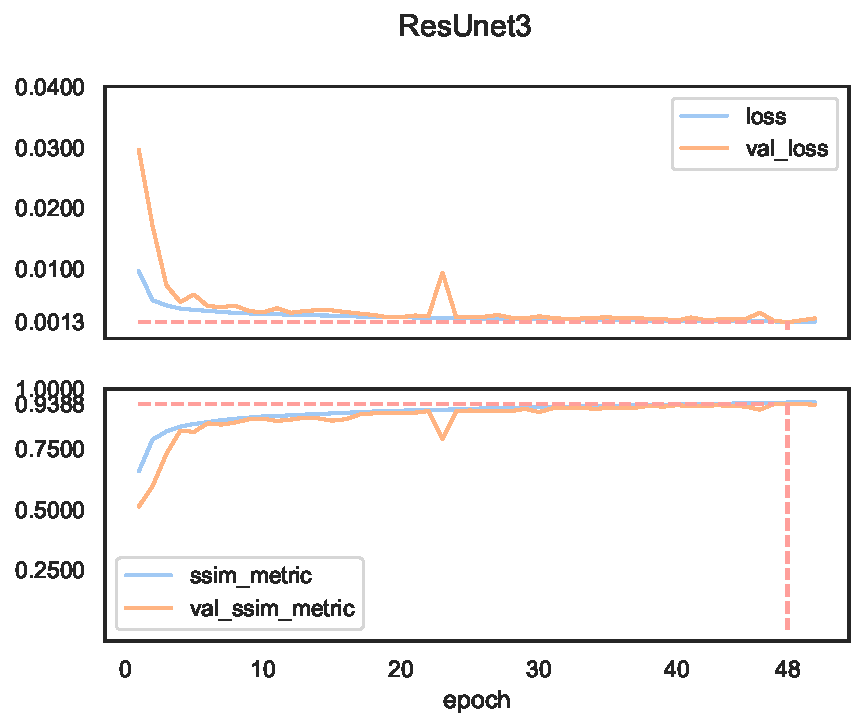
\includegraphics[height=0.4\textheight,keepaspectratio]{subsections/resunet/plot_history_ResUNet3.pdf}            
    \end{subfigure}
    \caption{Training information of ResUNet}
\end{figure}
 
\subsection{Results}
Two models were tested and the evaluation on a \textbf{uniform gaussian blur} is the following:
\begin{center}
    \small
    \begin{tabularx}{300pt}{cccc}
        \centering
        number of ResBlock & MSE & PSNR & SSIM \\
        1 & 0.0018 & 28.49 & 0.930 \\
        3 & 0.0016 & 29.03 & 0.935
    \end{tabularx}    
\end{center}

\begin{figure}[H]
    \centering
    {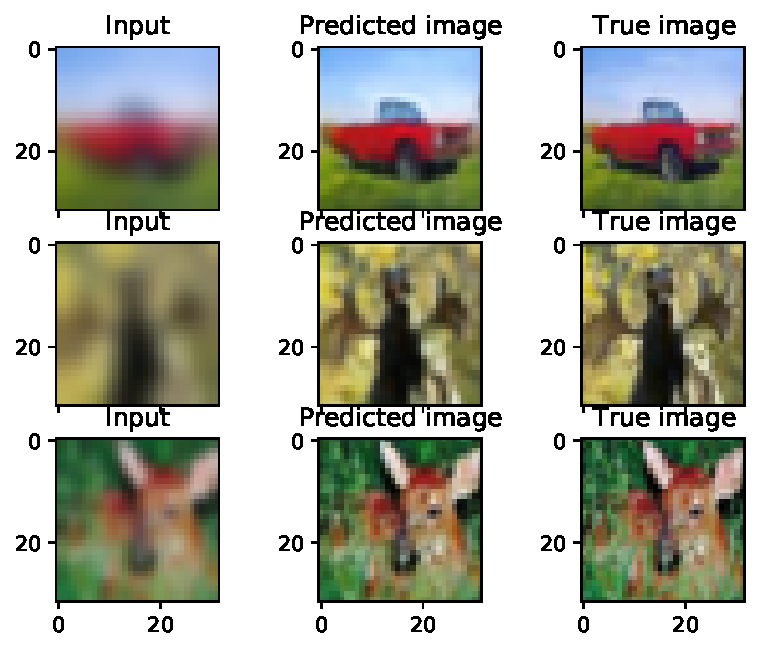
\includegraphics[height=0.35\textheight]{subsections/resunet/resunet1test.pdf}
    \caption{Test image generated by \textbf{ResUNet1}}}
    {\centering
    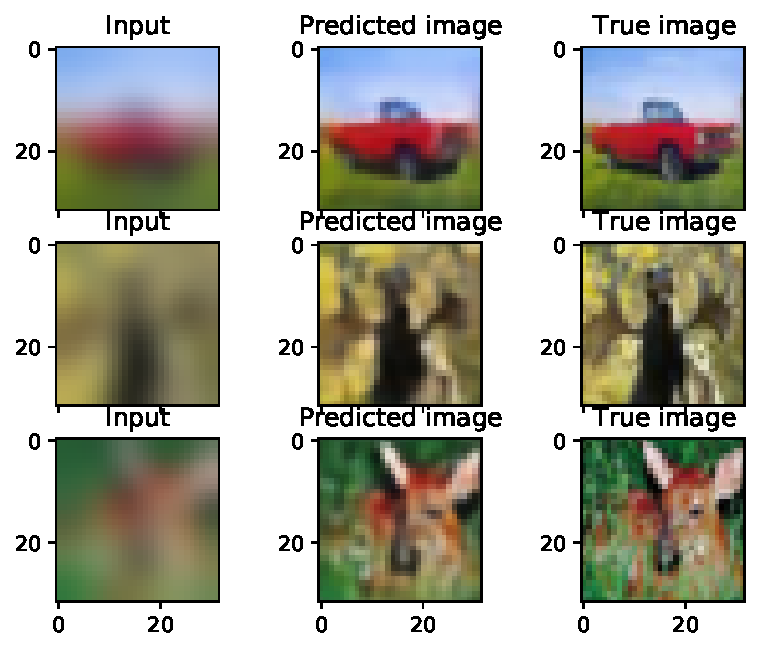
\includegraphics[height=0.35\textheight]{subsections/resunet/resunet3test.pdf}
    \caption{Test image generated by \textbf{ResUNet3}}}
\end{figure}

Both networks are able to generate quite sharp images but we can see that ResUnet3 is able to restore more fine details when the input is heavily blurred. 